In the previous Chapter, we demonstrated the use of the adjoint method to compute the gradient of a device that is parameterized by optical phase shifters.  We showed that this formalism allows one to train a common class of optical neural network based on MZI meshes.  In this Chapter, we will continue to explore the use of the adjoint method in training of optical machine learning hardware, but will take a more general approach.  Specifically, we will discuss the use of an optical system (or a wave system, more generally), as an analog computing platform for processing time series signals.  As we will show, this capability is made possible by the use of the adjoint method, which allows one to come up with a structure to solve a particular machine learning task through inverse design and optimization.

% In this framework, rather than using reflections or feedback circuits, the recurrence relationship occurs naturally in the time dynamics of the physics itself and the memory and information processing is provided by the waves as they propagate through space.

% To train the analog RNN, we show that standard gradient-based optimization techniques, as used in the field of machine learning, can tailor the physical characteristics of the system for a given task.
% This allows an inhomogeneous distribution of materials to learn complex features in time-series data with strong temporal dynamics.
% As a demonstration, we inject raw audio signals of spoken vowels into a numerical model of the wave equation and train the physical domain between the emitter and several receiving probes to classify the vowels.
% Our results demonstrate that such an approach can achieve high classification accuracy and is capable of generalizing to unseen vowel samples, with performance comparable to that of a conventional RNN.

\section{Wave Physics as a Recurrent Neural Network}

Analog computing platforms, which use the natural evolution of a continuous physical system to perform calculations, are emerging as important direction for the implementation of machine learning models \cite{shen_deep_2017, biamonte_quantum_2017, laporte2018numerical, lin2018all, khoram_stochastic_2018}.
Such a scheme has a number of potential benefits. Namely, they are able to \textit{passively} process signals and information in their native domain, without analog-to-digital conversion, which should result in a significant gain in speed and a reduction in power consumption.

Here, we identify a mapping between the dynamics of wave-based physical phenomena, such as acoustics and optics, and the computation in a recurrent neural network (RNN).
RNNs are one of the most important machine learning models and have been widely used to perform tasks such as natural language processing \cite{yao2013recurrent} and time-series prediction \cite{husken_recurrent_2003, dorffner_neural_1996, connor_recurrent_1994}.
Here we show that wave-based physical systems can be trained to operate as an RNN, and as a result can \textit{passively} process signals and information in their native domain, without analog-to-digital conversion, which should result in a significant gain in speed and a reduction in power consumption.

An RNN converts a sequence of inputs into a sequence of outputs by applying the same basic operation to each member of the input sequence in a step-by-step fashion (Fig \ref{fig:RNN}A). 
Memory of previous time steps is encoded into the RNN's \textit{hidden state}, which is updated at each step.
The information in the hidden state allows for the RNN to learn temporal structure and long-range dependencies in data \cite{elman1990finding, jordan1997serial}.
At a given time step, $t$, the RNN operates on the current input vector in the sequence, $\bvec{x}_t$, and the hidden state vector from the previous step, $\bvec{h}_{t-1}$, to produce an output vector, $\bvec{y}_t$, as well as an updated hidden state, $\bvec{h}_t$. 
%
While many variations of RNNs exist, a common implementation \cite{Goodfellow-et-al-2016} is described by the following update equations
%
\begin{align}
    \bvec{h}_t &= \sigh \left(\Wh \cdot \bvec{h}_{t-1} + \Wx \cdot \bvec{x}_t \right)
    \label{eq:RNN1} \\
    \bvec{y}_t &= \sigy \left(\Wy \cdot \bvec{h}_t\right),
    \label{eq:RNN2}
\end{align}
%
which are diagrammed in Fig. \ref{fig:RNN}B. 
As in the standard feedforward neural network case, the dense matrices defined by $\Wh$, $\Wx$, and $\Wy$ are optimized during training while $\sigh{\left(\cdot \right)}$ and $\sigy{\left(\cdot \right)}$ are fixed nonlinear activation functions.
The operation defined by Eq. \ref{eq:RNN1} and Eq. \ref{eq:RNN2}, when applied to each element of an input sequence, can be described by the directed graph shown in Fig. \ref{fig:RNN}C.

\begin{figure*}
  \centering
  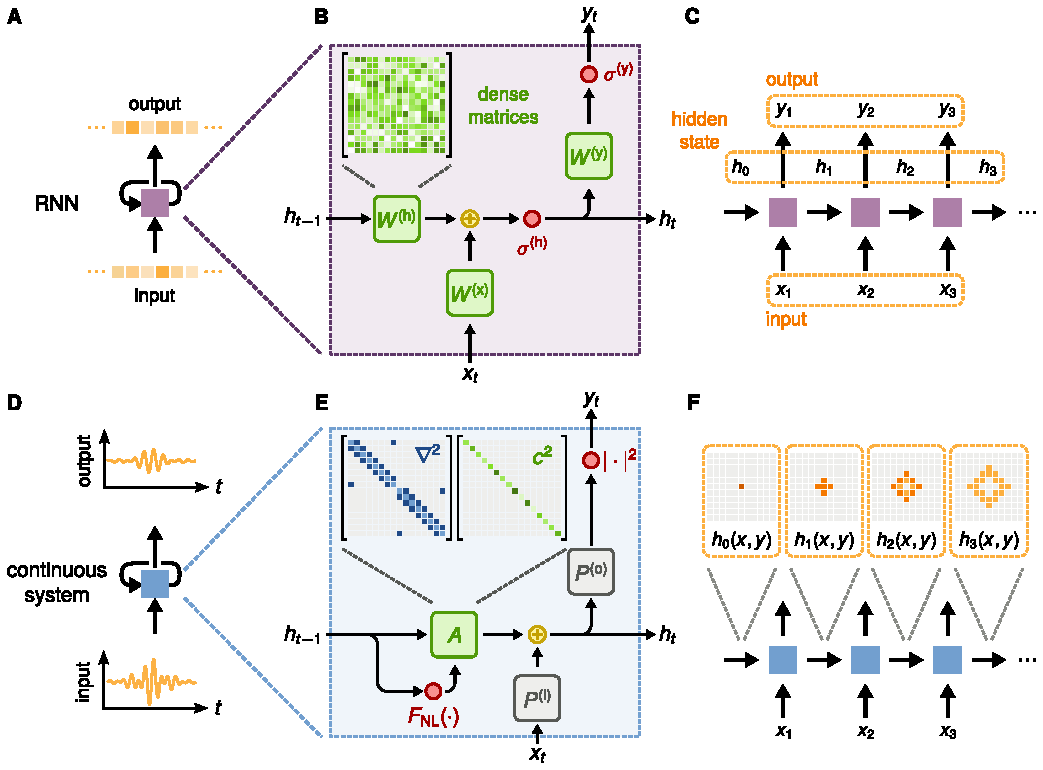
\includegraphics[width=\textwidth]{figures/insitu_RNN}
  \caption{
  \textbf{Conceptual comparison of a standard recurrent neural network and a wave-based physcal system.}
  (\textbf{A})
  Diagram of a recurrent neural network (RNN) cell operating on a discrete input sequence and producing a discrete output sequence. 
  (\textbf{B})
  Internal components of the RNN cell, consisting of trainable dense matrices $\Wh$, $\Wx$, and $\Wy$. 
  Activation functions for the hidden state and output are represented by $\sigh$ and $\sigy$, respectively. 
  (\textbf{C}) 
  Diagram of the directed graph of the RNN cell. 
  (\textbf{D}) 
  Diagram of a recurrent representation of a continuous physical system operating on a continuous input sequence and producing a continuous output sequence. 
  (\textbf{E}) 
  Internal components of the recurrence relation for the wave equation when discretized using finite differences. 
  (\textbf{F}) 
  Diagram of the directed graph of discrete time steps of the continuous physical system.}
  \label{fig:RNN}
\end{figure*}

We now discuss the connection between the dynamics in the RNN as described by Eqs. \ref{eq:RNN1} and \ref{eq:RNN2}, and the dynamics of a wave-based physical system.
We explore the dynamics of a scalar field distribution, $u = u{\left(x,y,z,t\right)}$, as governed by the damped wave equation \cite{elmore_physics_2012}
%
\begin{equation}
    \frac{\partial^2{u}}{{\partial{t}}^2} +  2 b \cdot \frac{\partial{u}}{{\partial{t}}} = c^2 \cdot \nabla^2 u + f,
    \label{eq:wave_eq_damping}
\end{equation}
where $\nabla^2 = \frac{\partial^2}{{\partial{x}}^2} + \frac{\partial^2}{{\partial{y}}^2} + \frac{\partial^2}{{\partial{z}}^2}$ is the Laplacian operator.
$c = c{\left(x,y,z\right)}$ is the spatial distribution of the wave speed and $f = f{\left(x,y,z,t\right)}$ is a source term.  
$b = c{\left(x,y,z\right)}$ is the dampening coefficient which is spatially varying but frequency-independent.
For a time step indexed by $t$, Eq. \ref{eq:wave_eq_damping} is discretized using \textit{centered} finite differences in time to give
\begin{align}
    \frac{u_{t+1} - 2u_t + u_{t-1}}{\Delta{t}^2} + 2b \frac{u_{t+1}-u_{t-1}}{2\Delta{t}} &= c^2 \nabla^2 u_t + f_t,
    \label{eq:wave_eq_damping_discretized}
\end{align}
where the subscript in $(\cdot)_t$ is used to indicate the value of a scalar field at time step $t$.

From Eq. \ref{eq:wave_eq_damping_discretized}, we may form a recurrence relation in terms of $u_{t+1}$, which leads to the following update equation
% \begin{widetext}
\begin{align}
    \left( \frac{1}{\Delta{t}^2} + \frac{b}{\Delta{t}}\right) u_{t+1} - \frac{2}{\Delta{t}^2} u_t  + \left( \frac{1}{\Delta{t}^2} - \frac{b}{\Delta{t}} \right) u_{t-1} = c^2 \cdot \nabla^2 u_t + f_t \nonumber \\
    \left( \frac{1}{\Delta{t}^2} + \frac{b}{\Delta{t}}\right) u_{t+1} = \frac{2}{\Delta{t}^2} u_t  - \left( \frac{1}{\Delta{t}^2} - \frac{b}{\Delta{t}} \right) u_{t-1} + c^2 \cdot\nabla^2 u_t + f_t \nonumber \\
    u_{t+1} = \left( \frac{1}{\Delta{t}^2} + \frac{b}{\Delta{t}}\right)^{-1} \left[ \frac{2}{\Delta{t}^2} u_t - \left( \frac{1}{\Delta{t}^2} - \frac{b}{\Delta{t}} \right) u_{t-1} + c^2\cdot \nabla^2 u_t + f_t \right].
    \label{eq:tmp1}
\end{align}
% \end{widetext}
Equation \ref{eq:tmp1} therefore represents the discretized update equation for the scalar wave equation with damping. In matrix form, we may express Eq. (\ref{eq:tmp1}) as
\begin{equation}
    \begin{bmatrix}
    u_{t+1} \\ u_t
    \end{bmatrix}
    = 
    \begin{bmatrix}
    \frac{2 + \Delta t^2\cdot c^2 \cdot \nabla^2}{1 + \Delta t\cdot b} 
    & \frac{-1 - \Delta t\cdot b}{1 + \Delta t\cdot b}  \\
    1 & 0
    \end{bmatrix}
    \cdot
    \begin{bmatrix}
    u_{t} \\ u_{t-1}
    \end{bmatrix}    
    +
    \Delta{t}^2 \cdot \begin{bmatrix}
     f_{t} \\ 0
    \end{bmatrix}.
    \label{eq:update_damped}
\end{equation}

Nonlinearity may be introduced into the system by assuming an intensity-dependent wave speed of the form $c{(x,y)} = c_{\text{linear}} + c_{\text{nonlinear}} \cdot \vert u_t{(x,y)} \vert^2$, where $c_{\text{nonlinear}}$ is exhibited in regions containing nonlinear materials.
In practice, this class of nonlinearity is encountered in a variety of wave physics, such as shallow water waves \cite{ursell_long-wave_1953} or nonlinear optics via the Kerr effect \cite{boyd_nonlinear_2008}.

To make the connection to the standard RNN more apparent, we define the wave system's \textit{hidden state} as the concatenation of the field distributions at the current and immediately preceding time steps, $\bvec{h}_t \equiv [\bvec{u}_t,~\bvec{u}_{t-1}]^T$, where $\bvec{u}_t$ and $\bvec{u}_{t-1}$ are vectors representing the \textit{flattened} fields, $u_t$ and $u_{t-1}$, discretized in the spatial domain.  With this, we may express the update of the wave equation from Eq. (\ref{eq:update_damped}) as
%
\begin{align}
\bvec{h}_t &= \bmat{A}{\left(\bvec{h}_{t-1}\right)} \cdot \bvec{h}_{t-1} + \Pin \cdot \bvec{x}_t \label{eq:sup_ScalarRNN1}\\
\bvec{y}_t &= \left\vert \Pout \cdot \bvec{h}_t \right\vert^2, \label{eq:sup_ScalarRNN2}
\end{align}
where we have defined $\bmat{A}$ as the matrix appearing in Eq. (\ref{eq:update_damped}) and its  dependence on $\bvec{h}_{t-1}$ is caused by the inclusion of the nonlinear wave speed as described above.

Like the standard RNN, the connections between the hidden state and the input and output of the wave equation are also defined by linear operators, given by $\Pin$ and $\Pout$. 
These matrices define injection and measuring points within the spatial domain.
Unlike the standard RNN, where the input and output matrices are dense, the input and output matrices of the wave equation are usually sparse and, moreover, unchanged by the training process.
The nonlinear relationship between the hidden state, $\bvec{h}_t$, and the output, $\bvec{y}_t$, of the wave equation is typical in wave physics since the output usually corresponds to a measurement of the wave intensity.

To more explicitly define the input and output of this RNN, we introduce the linear operators, $\Min$ and $\Mout$, each column of which define the respective spatial distributions of the injection and measurement points in this flattened basis.
With this, we can write the injection of the input vector ($\bvec{x}_t$) as a matrix-vector multiplication
%
\begin{equation}
    \Delta t^2 \bvec{f}_t \equiv \Min \cdot \bvec{x}_t.
\end{equation}

Similarly, as the output of the RNN at each time step is given by an intensity measurement of the scalar fields, we may express this in terms of the flattened scalar field as
\begin{equation}
    \bvec{y}_t = |\Mout{}^T \cdot \bvec{u}_t|^2.
\end{equation}

As the wave equation \textit{hidden state}, $\bvec{h}_t$ is defined as the concatenation of $\bvec{u}_t$ and $\bvec{u}_{t-1}$, we define the following matrices for convenience, as they only act on the $\bvec{u}_t$ portion of $\bvec{h}_t$
\begin{align}
    \Pin &\equiv \begin{bmatrix} \Min \\ \bmat{0} \end{bmatrix} \\ 
    \Pout &\equiv [\Mout{}^T,~\bmat{0}],
\end{align}
where $\bmat{0}$ is a matrix of all zeros.
These matrices are used in the injection and measurement stages of the scalar wave update equations of the main text and thus serve a similar role to the $\Wx$ and $\Wy$ matrices of the traditional RNN in Eqs. (\ref{eq:RNN1}) and (\ref{eq:RNN2}).  However, unlike $\Wx$ and $\Wy$, these matrices are fixed and not trainable parameters.

When training the system, we take the wave speed distribution, $c{\left(x,y,z\right)}$ as design parameters, which are optimized for a given machine learning task, physically corresponding to a patterning of materials within the domain.
Thus, when modeled numerically in discrete time (Fig. \ref{fig:RNN}E), the wave equation defines an operation which maps into that of an RNN (Fig. \ref{fig:RNN}B).
Similarly to the RNN, the full time dynamics of the wave equation may be represented as a directed graph (Fig. \ref{fig:RNN}F).

\begin{figure*}
  \centering
  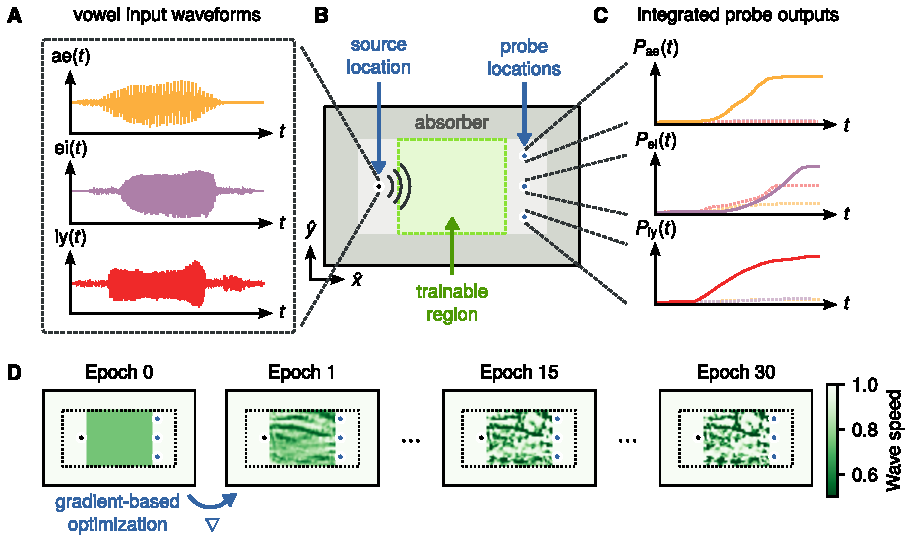
\includegraphics{figures/insitu_RNN_train}
  \caption{
  \textbf{Schematic of the vowel recognition system and the training procedure.}
  (\textbf{A})
  Raw audio waveforms of spoken vowel samples from three classes.
  (\textbf{B})
  Layout of the vowel recognition system. Vowel samples are independently injected at the source, located at the left of the domain, and propagate through the center region, indicated in green, where a material distribution is optimized during training. The dark gray region represents an absorbing boundary layer.
  (\textbf{C})
  For classification, the time-integrated power at each probe is measured and normalized to be interpreted as a probability distribution over the vowel classes.
  (\textbf{D})
  Using automatic differentiation, the gradient of the loss function with respect to the density of material in the green region is computed. The material density is updated iteratively, using gradient-based stochastic optimization techniques, until convergence.
  }
  \label{fig:train}
\end{figure*}

\section{Vowel Recognition Demonstration}

We now demonstrate how the dynamics of the wave equation can be trained to classify vowels through the construction of an inhomogeneous material distribution. 
For this task, we utilize a dataset consisting of 930 raw audio recordings of 10 vowel classes from 45 different male speakers and 48 different female speakers \cite{hillenbrand_acoustic_1995}.
For our learning task, we select a subset of 279 recordings corresponding to three vowel classes, represented by the vowel sounds \textit{ae}, \textit{ei}, and \textit{iy}, as contained in the words h\textit{a}d, h\textit{aye}d, and h\textit{ee}d, respectively (Fig. \ref{fig:train}A).
Before injection into the system, each vowel waveform is downsampled from its original recording with a 16 kHz sampling rate to a sampling rate of 10 kHz.

Our goal is to design a system such that when we inject the raw audio corresponding to each vowel (Fig. \ref{fig:train}A), the power is successfully directed to one of three measuring points.
The physical layout of the vowel recognition system consists of a two-dimensional domain in the $x$-$y$ plane, infinitely extended along the $z$-direction (Fig. \ref{fig:train}B). 
The audio waveform of each vowel, represented by $\bvec{x}^{(i)}$, is injected by a source at a single grid cell on the left side of the domain, emitting waveforms which propagate through a central region with a trainable distribution of the wave speed, indicated by the light green region in Fig. \ref{fig:train}B. 
An absorbing region is introduced to approximate an open boundary condition \cite{oskooi_failure_2008}, corresponding to the grey region in Fig. \ref{fig:train}B. 
This region is defined by a dampening coefficient, $b{(x,y)}$, which has a cubic dependence on the distance from the interior boundary of the layer.
The precense of absorption prevents energy from building up inside the computational domain.
Three probe points are defined on the right hand side of this region, each assigned to one of the three vowel classes. 
To determine the system's output, $\bvec{y}^{(i)}$, the time-integrated power at each probe is measured (Fig. \ref{fig:train}C). 
After the simulation evolves for the full duration of the vowel recording, this integral gives a non-negative vector of length 3, which is then normalized by its sum and interpreted as the system's predicted probability distribution over the vowel classes. 

For the purposes of our numerical demonstration, we consider binarized systems consisting of two materials: a background material with a normalized wave speed $c_0 = 1.0$, and a second material with $c_1 = 0.5$.
We assume that the second material has a nonlinear parameter, $c_{\text{nonlinear}} = -30$, while the background material has a linear response.
In practice, the wave speeds would be modified to correspond to different materials being used.
For example, in an acoustic setting the material distribution could consist of air, where the sound speed is 331 m/s, and porous silicone rubber, where the sound speed is 150 m/s \cite{ba_soft_2017}.
The initial distribution of the wave speed consists of a uniform region of material with a speed which is midway between those of the two materials (Fig. \ref{fig:train}D).

To create realistic devices with sufficiently large minimum feature sizes and binarized materials, we utilized spatial filtering and thresholding schemes.  A material density parameter $\rho(x,y)$ is defined for the structure, which may vary from 0 to 1.  Then, we apply a low pass spatial filter to $\rho(x,y)$, which gives a filtered density, labelled $\tilde{\rho}(x,y)$
%
% \begin{equation}
% \tilde{\rho}(x,y) = 
% \begin{bmatrix}
% 0.000 & 0.125 & 0.000 \\
% 0.125 & 0.500 & 0.125 \\
% 0.000 & 0.125 & 0.000
% \end{bmatrix}
% *
% \rho(x,y),
% \end{equation}
\begin{equation}
\tilde{\rho}(x,y) = 
\begin{bmatrix}
0 & 1/8 & 0 \\
1/8 & 1/2 & 1/8 \\
0 & 1/8 & 0
\end{bmatrix}
*
\rho(x,y).
\end{equation}
For binarization of the resulting structure, a projection scheme is used to recreate the final wave speed from the filtered density.  We define $\bar{\rho}(x,y)$ as the projected density, which is created from $\tilde{\rho}(x,y)$ as
\begin{equation}
\bar{\rho}_i = \frac{\tanh{\left( \beta \eta \right)} + \tanh{\left( \beta \left[ \tilde{\rho}_i - \eta \right] \right)}}{\tanh{\left( \beta \eta  \right)} + \tanh{\left( \beta \left[ 1 - \eta \right] \right)}}.
\end{equation}
Here, $\eta$ is a parameter between 0 and 1 that controls the mid-point of the projection, typically 0.5, and $\beta$ controls the strength of the projection, typically around 100.  The wave speed can be determined from $\bar{\rho}$ as
\begin{equation}
c(x,y) = (c_1(x,y) - c_0(x,y))\bar{\rho} + c_0(x,y),
\end{equation}
where $c_0$ and $c_1$ are the background and optimized material wave speed, respectively.

%

To train the system, we perform backpropagation through the model of the wave equation to compute the gradient of the cross entropy loss function of the measured outputs with respect to the density of material in each pixel of the trainable region.
As we discussed to in the previous Chapter, this process is mathematically equivalent performing the adjoint method.
Then, we use this gradient information update the material density using the the Adam optimization algorithm \cite{kingma2014adam}, repeating until convergence on a final structure (Fig. \ref{fig:train}D).

Numerical modeling and simulation of the wave equation physics was performed using a custom software package written in Python \cite{wavetorch}.
The software package was developed on top of the popular machine learning library, \texttt{pytorch}, to compute the gradients of the loss function with respect to the material distribution via reverse-mode automatic differentiation.
Using of a machine learning platform to perform the numerical simulation greatly reduces opportunities for errors in the analytic derivation or numerical implementation of the gradient. 

All windowed samples from the training set are run through the simulation in batches of 9 and the categorical cross entropy loss between the output probe probability distribution and the correct one-hot vector for each vowel sample is computed.
To encourage the optimizer to produce a binarized distribution of the wave speed with relatively large feature sizes, the optimizer minimizes this loss function with respect to a material density distribution, $\rho{\left(x,y\right)}$ within a central region of the simulation domain, indicated by the green region in Fig. \ref{fig:train}B. 
We use the Adam algorithm \cite{kingma_adam_2014} with learning rate 0.0004 to perform the optimization in batches of 9.
Fig. \ref{fig:train}D illustrates the optimization process over several epochs, during which, the wave velocity distribution converges to a final structure.
At the end of each epoch, the classification accuracy is computed over both the testing and training set. 
Unlike the training set, the full length of each vowel sample from the testing set is used.

The mean energy spectrum of the three vowel classes after downsampling to 10 kHz is shown in Fig. \ref{fig:s_spectrum}.
We observe that the majority of the energy for all vowel classes is below 1 kHz and that there is strong overlap between the mean peak energy of the \textit{ei} and \textit{iy} vowel classes.
Moreover, the mean peak energy of the \textit{ae} vowel class is very close to the peak energy of the other two vowels.
Therefore, the vowel recognition task learned by the system in the main text is non-trivial.

\begin{figure*}[t]
  \centering
  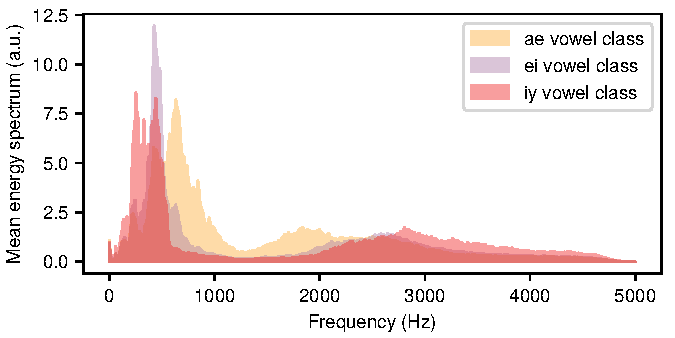
\includegraphics{figures/insitu_spectrum}
  \caption{Mean energy spectrum for the \textit{ae}, \textit{ei}, and \textit{iy} vowel classes.}
  \label{fig:s_spectrum}
\end{figure*}

To validate the performance of our system, the full dataset of (3 classes) $\times$ (45 males + 48 females) = 272 vowel samples is divided into 5 groups of approximately equal size.
Cross validated training is performed with 4 out of the 5 sample groups forming a training set and 1 out of the 5 sample groups forming a testing set.
Independent training runs are performed with each of the 5 groups serving as the testing set, with results being averaged over all training runs. 
During each epoch, every sample vowel sequence from the training set is windowed to a length of 1000, taken from the center of the sequence, but the testing is performed on the full sequence.

% 4. What are the limitations?
% One major limitation of our approach is that it relies on numerical simulation for training, which may be an issue when the simulation size becomes too complex to model feasibly on a digital computer.  
% Furthermore, the presence of chaos or high sensitivity to inputs and initial conditions in the system may introduce significant differences between the numerical simulation and the physical realization, meaning that the digitally trained device may not perform as expected when fabricated and introduced to physical signals.
% However, this issue may be mitigated by utilizing the previously mentioned techniques from the field of inverse design, such as fabrication or sensitivity constraints \cite{wang2011robust, piggott2017fabrication}.

% \section{Binarization and Filtering of Wave Speed \label{appx:fab}}

The confusion matrices over the training and testing sets for the starting structure are shown in Fig. \ref{fig:results}A and Fig. \ref{fig:results}B, averaged over five cross-validated training runs.
Here, the confusion matrix defines the percentage of correctly predicted vowels along its diagonal entries and the percentage of incorrectly predicted vowels for each class in its off-diagonal entries.
Clearly the starting structure can not perform the recognition task.
Fig. \ref{fig:results}C and Fig. \ref{fig:results}D show the final confusion matrices after optimization for the testing and training sets, averaged over five cross validated training runs.
The trained confusion matrices are diagonally dominant, indicating that the structure can indeed perform vowel recognition.

Fig. \ref{fig:results}E and Fig. \ref{fig:results}F show the cross entropy loss value and the prediction accuracy, respectively, as a function of the training epoch over the testing and training datasets, where the solid line indicates the mean and the shaded region corresponds to the standard deviation over the cross-validated training runs.
Interestingly, we observe that the first epoch results in the largest reduction of the loss function and the largest gain in prediction accuracy.
From Fig. \ref{fig:results}F we see that the system obtains a mean accuracy of 92.6\% $\pm$ 1.1\% over the training dataset and a mean accuracy of 86.3\% $\pm$ 4.3\% over the testing dataset.
From Fig. \ref{fig:results}C and Fig. \ref{fig:results}D we observe that the system attains near perfect prediction performance on the \textit{ae} vowel and is able to differentiate the \textit{iy} vowel from the \textit{ei} vowel, but with less accuracy, especially in unseen samples from the testing dataset. 
Fig. \ref{fig:results}G, Fig. \ref{fig:results}H, and Fig. \ref{fig:results}I show the distribution of the integrated field intensity, $\sum_t{\left\vert u_t{\left(x,y\right)} \right\vert^2}$, when a representative sample from each vowel class is injected into the trained structure. 
We thus provide visual confirmation that the optimization procedure produces a structure which routes the majority of the signal energy to the correct probe. 
As a performance benchmark, a conventional RNN was trained on the same task, achieving comparable classification accuracy to that of the wave equation. However, a larger number of free parameters was required.
Additionally, we observed that a comparable classification accuracy was obtained when training a linear wave equation.

\begin{figure*}
  \centering
  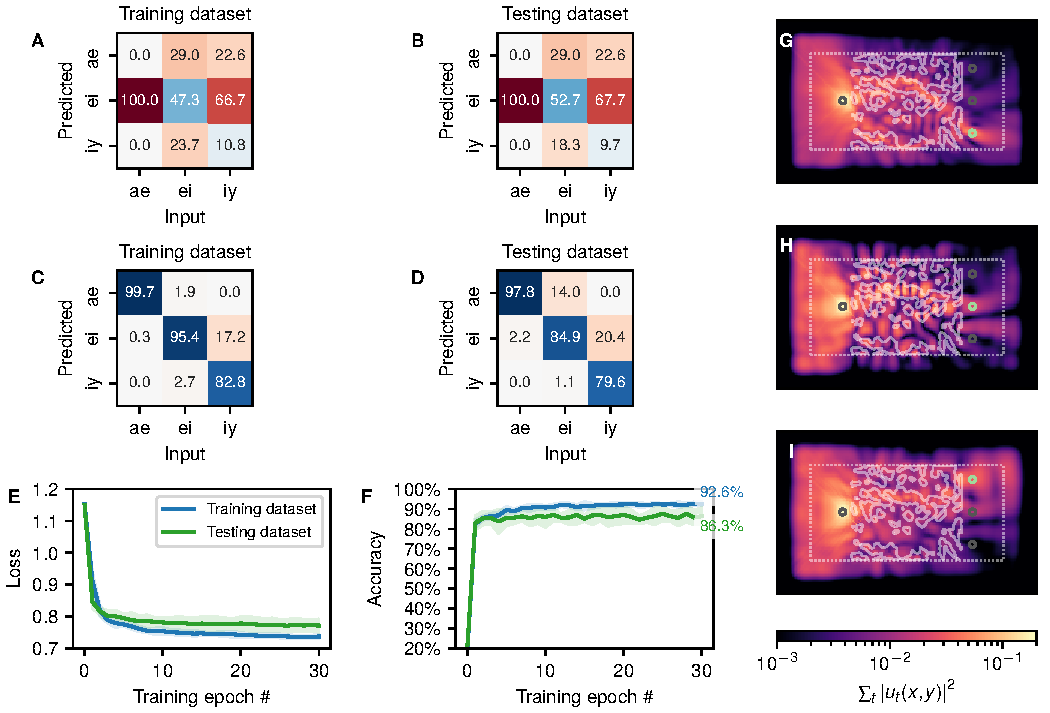
\includegraphics[width=\textwidth]{figures/insitu_RNN_results}
  \caption{\textbf{Vowel recognition system training results.}
  Confusion matrix over the training and testing datasets for the initial structure (\textbf{A}),(\textbf{B}) and final structure (\textbf{C}),(\textbf{D}), indicating the percentage or correct (diagonal) and incorrect (off-diagonal). 
  Cross validated training results showing the mean (sold line) and standard deviation (shaded region) of the (\textbf{E}) cross entropy loss and (\textbf{F}) prediction accuracy over 20 training epochs and 5 folds of the dataset, which consists of a total of 272 total vowel samples of male and female speakers.
  (\textbf{G})-(\textbf{I}) The time-integrated intensity distribution for a randomly selected input (\textbf{G}) \textit{ae} vowel, (\textbf{H}) \textit{ei} vowel, and (\textbf{I}) \textit{iy} vowel.}
  \label{fig:results}
\end{figure*}

We compare the wave equation results to a conventional RNN model as defined in Eq. (\ref{eq:RNN1}) and Eq. (\ref{eq:RNN2}). 
The number of trainable parameters in the model is determined by the hidden state size $N_h$, as the model is given by three matrices $\Wx, \Wh$, and $\Wy$ of size $[N_h, 1]$, $[N_h, N_h]$ and $[3, N_h]$, respectively. 
We tried $N_h = $70, for which the total number of RNN free parameters is 5250, and $N_h=$100, with 10500 free parameters. 
The RNN was implemented and trained using \texttt{pytorch}.  
In Table \ref{tab:final_table} we show the results of a standard RNN on the vowel recognition task and compare them to the scalar wave.  
We find that the conventional RNN achieves a performance comparable to the wave equation.
However, this performance is highly dependent on the number of trainable parameters.  
For a similar number of trainable parameters, the conventional RNN achieves about 6\% lower classification accuracy.  
However, when the number of free parameters is increased to about 2 times that of the scalar wave, the accuracy is higher by about 3 \%. 
We note that it is possible that more advanced recurrent models like long short-term memory (LSTM) \cite{hochreiter1997long} or gated recurrent unit (GRU) \cite{chung2014empirical} could have a better performance with a smaller number of parameters, but exploring this is outside the scope of this study. 

\begin{table*}[t]
    \centering
    \setlength{\tabcolsep}{6pt}
    \renewcommand{\arraystretch}{1.25}
    \begin{tabular}{llccccc}
        \hline\hline
        \textbf{Model} & \textbf{Nonlinearity} & \textbf{\# parameters} & \multicolumn{2}{c}{\textbf{Accuracy}} \\
        & & & Training & Testing \\
        \hline
        \textbf{Wave Equation} & linear wave speed & 4200 & 93.1\% & 86.6\% \\
          & nonlinear wave speed & 4200 & 92.6\% & 86.3\% \\
%       \hline
        \hline
        \textbf{Conventional RNN} & linear & 5250 & 78.8\% & 79.4\% \\
        & leaky ReLU & 5250 & 82.6\% & 80.2\% \\
%       \hline
        & linear & 10500  & 88.9\% & 88.2\% \\
        & leaky ReLU     & 10500 & 89.4\% & 89.4\% \\
        \hline\hline
    \end{tabular}
    \caption{Comparison of scalar wave model and conventional RNN on vowel recognition task.}
    \label{tab:final_table}
\end{table*}

\section{Comparison of Analog and Digital Implementations}

The conventional RNN and the one implemented by a scalar wave equation have many qualitative differences.
We discuss some of those below. 
First, in the RNN case, the trainable parameters are given by the elements of the weight matrices.  
In the wave equation case, we choose to use the wave velocity, $c(x,y,z)$, as trainable parameters, because a specific distribution of $c$ can be physically implemented after the training process.  
In acoustic or optical systems, this can be practically realized using technologies such as 3D printing or nanolithography. 
Furthermore, whereas the RNN free parameters define a matrix which is multiplied by the input, output, and hidden state vectors, in the wave equation case, the free parameters are multiplied element-wise with the hidden state, which limits the influence of each individual parameter over the full dynamics.  

% \subsection{Length and Time Scale}

For a given amount of expressive power, the size of the hidden state in the wave equation must arguably be much larger than that in the RNN case.  This is because the amount of information that can be encoded in the spatial distribution of $u_t$ is constrained by the diffraction limit for wave systems.  It follows that a single RNN hidden state element may be analogous to several grid cells in the scalar wave equation. Furthermore, the wave update matrix $A$ is sparse and only contains non-zeros on diagonal elements (self coupling) and those corresponding to neighbor-to-neighbor coupling between spatial grid cells.  Because of this, information in a given cell of $u_t$ will take several time steps to reach other cells, as determined by the wave velocity and the distance between them.  The presence of this form of causality practically means that one must wait longer for a full `mixing' of information between cells in the domain, suggesting that in the our numerical simulations, a larger number of time steps may be needed as compared to the typical RNN. 

% \subsection{Nonlinearities}  

The form of nonlinearity used in the wave equation is different from that in the typical RNN, which involves the application of the nonlinear function, $\sigh(\cdot)$, as in Eq. (\ref{eq:RNN1}).  In the wave equation, nonlinearity is provided by making the wave velocity, $c$, or damping dependent, $b$, to be dependent on the instantaneous wave intensity $|u_t|^2$.  For example $c = c(|u_t|^2)$, or $b = b(|u_t|^2)$.  In optics, these nonlinearities may be implemented using $\chi^{(3)}$ materials or saturable absorption, respectively.  With this addition, the update matrix of Eq. (\ref{eq:sup_ScalarRNN1}), $\bmat{A} = \bmat{A}(\bvec{h}_{t-1})$, becomes a function of the solution at that time step, making the dynamics nonlinear.  Nonlinearity is introduced into the  output of the wave system ($\bvec{y}_t$) by measuring the intensity of the wave field, which involves a squaring operation.  One may also consider directly discretizing a nonlinear wave equation using the same technique.

The wave-based RNN presented here has a number of favorable qualities that make it a good candidate for processing sequential data.
Unlike the standard RNN, the update of the wave equation from one time step to the next enforces a nearest-neighbor coupling between elements of the hidden state through the Laplacian operator, which is represented by a sparse matrix in Fig. \ref{fig:RNN}E. 
This is a direct consequence of the fact that the wave equation is a hyperbolic partial differential equation in which information propagates with a finite velocity. 
Thus, the size of the analog RNN's hidden state, and therefore its memory capacity, is directly determined by the size of the propagation medium. 
Additionally, unlike the conventional RNN, the wave equation enforces an energy conservation constraint, preventing unbounded growth of the norm of the hidden state and the output signal.
In contrast, the unconstrained dense matrices defining the update relationship of the standard RNN lead to vanishing and exploding gradients, which pose a major challenge for training traditional RNNs \cite{jing2017tunable}.

In this chapter, we have shown that the dynamics of the wave equation are conceptually equivalent to those of a recurrent neural network.
This conceptual connection opens up the opportunity for a new class of analog hardware platform, in which evolving time dynamics play a significant role in both the physics and the dataset.
% Our results also demonstrate that inverse design techniques are effective at training physical systems on machine learning tasks.
% In particular, we demonstrated that, on a vowel classification problem, train and test accuracies of \result{93}\% and \result{86}\% can be attained, which are comparable to those from a standard RNN with a comparable number of free parameters.
% More broadly, our results point toward several exciting directions in analog computing for machine learning.
While we have focused on a specific example of the scalar wave equation, our results apply broadly to other wave-like physics.
Such an approach of using physics to perform computation \cite{silva_performing_2014, hermans_trainable_2015, guo_photonic_2018, lin2018all, kwon_nonlocal_2018, estakhri_inverse-designed_2019} may inspire a new platform for analog machine learning devices, with the potential to perform computation far more naturally and efficiently than their digital counterparts.
The generality of the approach further suggests that many physical systems may be attractive candidates for performing RNN-like computation on naturally occurring sequences, such as optical, acoustic, or seismic signals.
